\documentclass[twoside]{book}

% Packages required by doxygen
\usepackage{fixltx2e}
\usepackage{calc}
\usepackage{doxygen}
\usepackage[export]{adjustbox} % also loads graphicx
\usepackage{graphicx}
\usepackage[utf8]{inputenc}
\usepackage{makeidx}
\usepackage{multicol}
\usepackage{multirow}
\PassOptionsToPackage{warn}{textcomp}
\usepackage{textcomp}
\usepackage[nointegrals]{wasysym}
\usepackage[table]{xcolor}

% NLS support packages
\usepackage[T2A]{fontenc}
\usepackage[russian]{babel}

% Font selection
\usepackage[T1]{fontenc}
\usepackage[scaled=.90]{helvet}
\usepackage{courier}
\usepackage{amssymb}
\usepackage{sectsty}
\renewcommand{\familydefault}{\sfdefault}
\allsectionsfont{%
  \fontseries{bc}\selectfont%
  \color{darkgray}%
}
\renewcommand{\DoxyLabelFont}{%
  \fontseries{bc}\selectfont%
  \color{darkgray}%
}
\newcommand{\+}{\discretionary{\mbox{\scriptsize$\hookleftarrow$}}{}{}}

% Page & text layout
\usepackage{geometry}
\geometry{%
  a4paper,%
  top=2.5cm,%
  bottom=2.5cm,%
  left=2.5cm,%
  right=2.5cm%
}
\tolerance=750
\hfuzz=15pt
\hbadness=750
\setlength{\emergencystretch}{15pt}
\setlength{\parindent}{0cm}
\setlength{\parskip}{3ex plus 2ex minus 2ex}
\makeatletter
\renewcommand{\paragraph}{%
  \@startsection{paragraph}{4}{0ex}{-1.0ex}{1.0ex}{%
    \normalfont\normalsize\bfseries\SS@parafont%
  }%
}
\renewcommand{\subparagraph}{%
  \@startsection{subparagraph}{5}{0ex}{-1.0ex}{1.0ex}{%
    \normalfont\normalsize\bfseries\SS@subparafont%
  }%
}
\makeatother

% Headers & footers
\usepackage{fancyhdr}
\pagestyle{fancyplain}
\fancyhead[LE]{\fancyplain{}{\bfseries\thepage}}
\fancyhead[CE]{\fancyplain{}{}}
\fancyhead[RE]{\fancyplain{}{\bfseries\leftmark}}
\fancyhead[LO]{\fancyplain{}{\bfseries\rightmark}}
\fancyhead[CO]{\fancyplain{}{}}
\fancyhead[RO]{\fancyplain{}{\bfseries\thepage}}
\fancyfoot[LE]{\fancyplain{}{}}
\fancyfoot[CE]{\fancyplain{}{}}
\fancyfoot[RE]{\fancyplain{}{\bfseries\scriptsize Создано системой Doxygen }}
\fancyfoot[LO]{\fancyplain{}{\bfseries\scriptsize Создано системой Doxygen }}
\fancyfoot[CO]{\fancyplain{}{}}
\fancyfoot[RO]{\fancyplain{}{}}
\renewcommand{\footrulewidth}{0.4pt}
\renewcommand{\chaptermark}[1]{%
  \markboth{#1}{}%
}
\renewcommand{\sectionmark}[1]{%
  \markright{\thesection\ #1}%
}

% Indices & bibliography
\usepackage{natbib}
\usepackage[titles]{tocloft}
\setcounter{tocdepth}{3}
\setcounter{secnumdepth}{5}
\makeindex

% Hyperlinks (required, but should be loaded last)
\usepackage{ifpdf}
\ifpdf
  \usepackage[pdftex,pagebackref=true]{hyperref}
\else
  \usepackage[ps2pdf,pagebackref=true]{hyperref}
\fi
\hypersetup{%
  colorlinks=true,%
  linkcolor=blue,%
  citecolor=blue,%
  unicode%
}

% Custom commands
\newcommand{\clearemptydoublepage}{%
  \newpage{\pagestyle{empty}\cleardoublepage}%
}

\usepackage{caption}
\captionsetup{labelsep=space,justification=centering,font={bf},singlelinecheck=off,skip=4pt,position=top}

%===== C O N T E N T S =====

\begin{document}

% Titlepage & ToC
\hypersetup{pageanchor=false,
             bookmarksnumbered=true,
             pdfencoding=unicode
            }
\pagenumbering{roman}
\begin{titlepage}
\vspace*{7cm}
\begin{center}%
{\Large Simple Plotter Widget for QT \\[1ex]\large 1.\+0 }\\
\vspace*{1cm}
{\large Создано системой Doxygen 1.8.11}\\
\end{center}
\end{titlepage}
\clearemptydoublepage
\tableofcontents
\clearemptydoublepage
\pagenumbering{arabic}
\hypersetup{pageanchor=true}

%--- Begin generated contents ---
\chapter{Иерархический список классов}
\section{Иерархия классов}
Иерархия классов.\begin{DoxyCompactList}
\item Q\+Exception\begin{DoxyCompactList}
\item \contentsline{section}{Simple\+Plotter\+Exception}{\pageref{class_simple_plotter_exception}}{}
\end{DoxyCompactList}
\item Q\+Graphics\+Scene\begin{DoxyCompactList}
\item \contentsline{section}{Simple\+Plotter\+Scene}{\pageref{class_simple_plotter_scene}}{}
\end{DoxyCompactList}
\item Q\+Graphics\+View\begin{DoxyCompactList}
\item \contentsline{section}{Simple\+Plotter\+View}{\pageref{class_simple_plotter_view}}{}
\end{DoxyCompactList}
\item Q\+Main\+Window\begin{DoxyCompactList}
\item \contentsline{section}{Main\+Window}{\pageref{class_main_window}}{}
\end{DoxyCompactList}
\item Q\+Widget\begin{DoxyCompactList}
\item \contentsline{section}{Simple\+Plotter\+Widget}{\pageref{class_simple_plotter_widget}}{}
\end{DoxyCompactList}
\item \contentsline{section}{Simple2\+D\+Plot}{\pageref{class_simple2_d_plot}}{}
\end{DoxyCompactList}

\chapter{Алфавитный указатель классов}
\section{Классы}
Классы с их кратким описанием.\begin{DoxyCompactList}
\item\contentsline{section}{\hyperlink{class_main_window}{Main\+Window} }{\pageref{class_main_window}}{}
\item\contentsline{section}{\hyperlink{class_simple2_d_plot}{Simple2\+D\+Plot} \\*�����, �������� ���������� � ������� }{\pageref{class_simple2_d_plot}}{}
\item\contentsline{section}{\hyperlink{class_simple_plotter_exception}{Simple\+Plotter\+Exception} \\*����� ���������� }{\pageref{class_simple_plotter_exception}}{}
\item\contentsline{section}{\hyperlink{class_simple_plotter_scene}{Simple\+Plotter\+Scene} }{\pageref{class_simple_plotter_scene}}{}
\item\contentsline{section}{\hyperlink{class_simple_plotter_view}{Simple\+Plotter\+View} \\*�������� ����� ������� }{\pageref{class_simple_plotter_view}}{}
\item\contentsline{section}{\hyperlink{class_simple_plotter_widget}{Simple\+Plotter\+Widget} }{\pageref{class_simple_plotter_widget}}{}
\end{DoxyCompactList}

\chapter{Классы}
\hypertarget{class_main_window}{}\section{Класс Main\+Window}
\label{class_main_window}\index{Main\+Window@{Main\+Window}}
Граф наследования\+:Main\+Window\+:\begin{figure}[H]
\begin{center}
\leavevmode
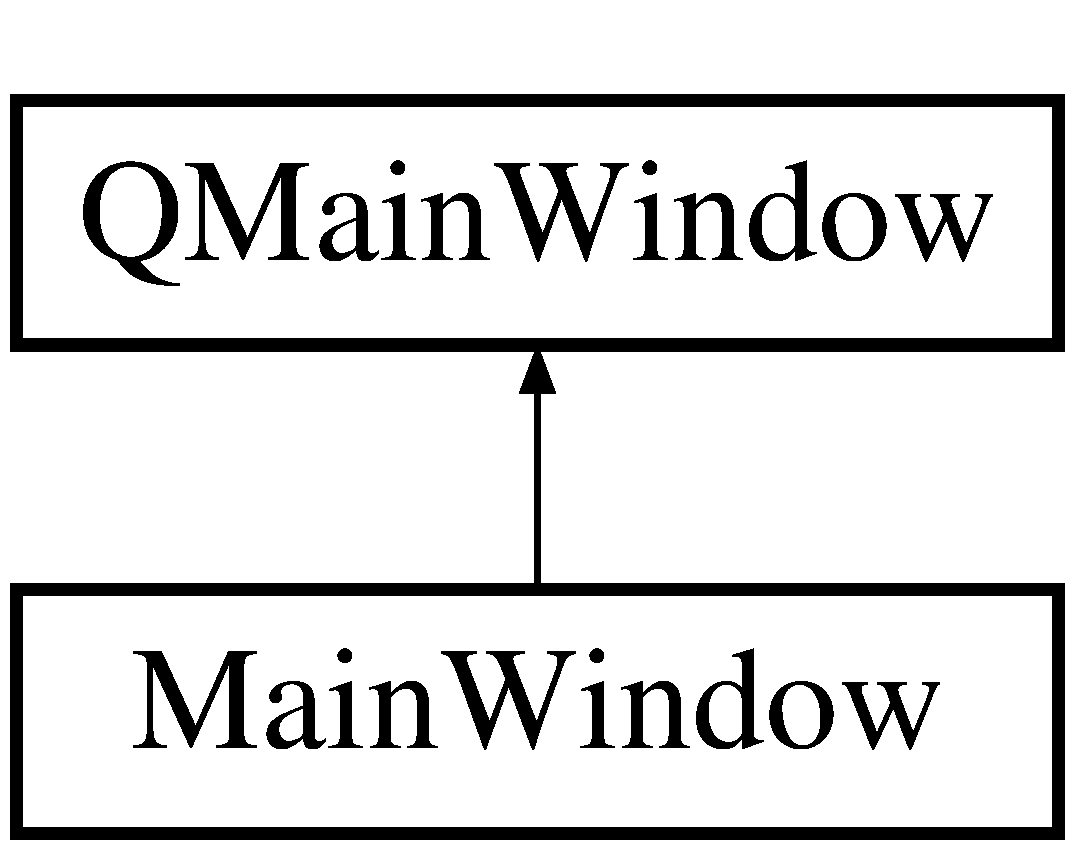
\includegraphics[height=2.000000cm]{class_main_window}
\end{center}
\end{figure}
\subsection*{Открытые члены}
\begin{DoxyCompactItemize}
\item 
{\bfseries Main\+Window} (Q\+Widget $\ast$parent=0)\hypertarget{class_main_window_a8b244be8b7b7db1b08de2a2acb9409db}{}\label{class_main_window_a8b244be8b7b7db1b08de2a2acb9409db}

\end{DoxyCompactItemize}


Объявления и описания членов классов находятся в файлах\+:\begin{DoxyCompactItemize}
\item 
mainwindow.\+h\item 
mainwindow.\+cpp\end{DoxyCompactItemize}

\hypertarget{class_simple2_d_plot}{}\section{Класс Simple2\+D\+Plot}
\label{class_simple2_d_plot}\index{Simple2\+D\+Plot@{Simple2\+D\+Plot}}


�����, �������� ���������� � �������  




{\ttfamily \#include $<$simple2dplot.\+h$>$}

\subsection*{Открытые члены}
\begin{DoxyCompactItemize}
\item 
\hyperlink{class_simple2_d_plot_a74b70aa66b161adf0c464b123fb80338}{Simple2\+D\+Plot} (std\+::string name, Q\+Vector$<$ Q\+Point $>$ points)
\begin{DoxyCompactList}\small\item\em ����������� �� ������� �����. \end{DoxyCompactList}\item 
\hyperlink{class_simple2_d_plot_ad3dc6487722709085782540894020328}{Simple2\+D\+Plot} (std\+::string name, std\+::function$<$ double(double)$>$ func, double lower, double upper, double step)
\begin{DoxyCompactList}\small\item\em ����������� �� �������. \end{DoxyCompactList}\item 
{\footnotesize template$<$typename T $>$ }\\\hyperlink{class_simple2_d_plot_ad143bd7f095b88695354b10a4ebc0d07}{Simple2\+D\+Plot} (std\+::string name, Q\+Vector$<$ Q\+Pair$<$ T, T $>$ $>$ points)
\begin{DoxyCompactList}\small\item\em ����������� �� ������ ����� \end{DoxyCompactList}\item 
std\+::string \hyperlink{class_simple2_d_plot_a15e3412379e8a799871e274f3140b4b4}{get\+Name} () const 
\begin{DoxyCompactList}\small\item\em ���������� ��� \end{DoxyCompactList}\item 
points\+Vector \hyperlink{class_simple2_d_plot_a76cd841505fd2db3d1b2c57987e5375c}{get\+Points} () const 
\begin{DoxyCompactList}\small\item\em ���������� ������ ����� \end{DoxyCompactList}\end{DoxyCompactItemize}


\subsection{Подробное описание}
�����, �������� ���������� � ������� 

\subsection{Конструктор(ы)}
\index{Simple2\+D\+Plot@{Simple2\+D\+Plot}!Simple2\+D\+Plot@{Simple2\+D\+Plot}}
\index{Simple2\+D\+Plot@{Simple2\+D\+Plot}!Simple2\+D\+Plot@{Simple2\+D\+Plot}}
\subsubsection[{\texorpdfstring{Simple2\+D\+Plot(std\+::string name, Q\+Vector$<$ Q\+Point $>$ points)}{Simple2DPlot(std::string name, QVector< QPoint > points)}}]{\setlength{\rightskip}{0pt plus 5cm}Simple2\+D\+Plot\+::\+Simple2\+D\+Plot (
\begin{DoxyParamCaption}
\item[{std\+::string}]{name, }
\item[{Q\+Vector$<$ Q\+Point $>$}]{points}
\end{DoxyParamCaption}
)}\hypertarget{class_simple2_d_plot_a74b70aa66b161adf0c464b123fb80338}{}\label{class_simple2_d_plot_a74b70aa66b161adf0c464b123fb80338}


����������� �� ������� �����. 


\begin{DoxyParams}{Аргументы}
{\em name} & �������� ������� \\
\hline
{\em points} & ������ ����� \\
\hline
\end{DoxyParams}
\index{Simple2\+D\+Plot@{Simple2\+D\+Plot}!Simple2\+D\+Plot@{Simple2\+D\+Plot}}
\index{Simple2\+D\+Plot@{Simple2\+D\+Plot}!Simple2\+D\+Plot@{Simple2\+D\+Plot}}
\subsubsection[{\texorpdfstring{Simple2\+D\+Plot(std\+::string name, std\+::function$<$ double(double)$>$ func, double lower, double upper, double step)}{Simple2DPlot(std::string name, std::function< double(double)> func, double lower, double upper, double step)}}]{\setlength{\rightskip}{0pt plus 5cm}Simple2\+D\+Plot\+::\+Simple2\+D\+Plot (
\begin{DoxyParamCaption}
\item[{std\+::string}]{name, }
\item[{std\+::function$<$ double(double)$>$}]{func, }
\item[{double}]{lower, }
\item[{double}]{upper, }
\item[{double}]{step}
\end{DoxyParamCaption}
)}\hypertarget{class_simple2_d_plot_ad3dc6487722709085782540894020328}{}\label{class_simple2_d_plot_ad3dc6487722709085782540894020328}


����������� �� �������. 


\begin{DoxyParams}{Аргументы}
{\em name} & �������� ������� \\
\hline
{\em func} & ������� double -\/$>$ double \\
\hline
{\em lower} & ������ ������� \\
\hline
{\em upper} & ������� ������� \\
\hline
{\em step} & ��� \\
\hline
\end{DoxyParams}
\index{Simple2\+D\+Plot@{Simple2\+D\+Plot}!Simple2\+D\+Plot@{Simple2\+D\+Plot}}
\index{Simple2\+D\+Plot@{Simple2\+D\+Plot}!Simple2\+D\+Plot@{Simple2\+D\+Plot}}
\subsubsection[{\texorpdfstring{Simple2\+D\+Plot(std\+::string name, Q\+Vector$<$ Q\+Pair$<$ T, T $>$ $>$ points)}{Simple2DPlot(std::string name, QVector< QPair< T, T > > points)}}]{\setlength{\rightskip}{0pt plus 5cm}template$<$typename T $>$ template$<$ typename T $>$ Simple2\+D\+Plot\+::\+Simple2\+D\+Plot (
\begin{DoxyParamCaption}
\item[{std\+::string}]{name, }
\item[{Q\+Vector$<$ Q\+Pair$<$ T, T $>$ $>$}]{points}
\end{DoxyParamCaption}
)}\hypertarget{class_simple2_d_plot_ad143bd7f095b88695354b10a4ebc0d07}{}\label{class_simple2_d_plot_ad143bd7f095b88695354b10a4ebc0d07}


����������� �� ������ ����� 


\begin{DoxyParams}{Аргументы}
{\em name} & �������� ������� \\
\hline
{\em points} & ������ ����� � ���� ��� x, y \\
\hline
\end{DoxyParams}


\subsection{Методы}
\index{Simple2\+D\+Plot@{Simple2\+D\+Plot}!get\+Name@{get\+Name}}
\index{get\+Name@{get\+Name}!Simple2\+D\+Plot@{Simple2\+D\+Plot}}
\subsubsection[{\texorpdfstring{get\+Name() const }{getName() const }}]{\setlength{\rightskip}{0pt plus 5cm}std\+::string Simple2\+D\+Plot\+::get\+Name (
\begin{DoxyParamCaption}
{}
\end{DoxyParamCaption}
) const}\hypertarget{class_simple2_d_plot_a15e3412379e8a799871e274f3140b4b4}{}\label{class_simple2_d_plot_a15e3412379e8a799871e274f3140b4b4}


���������� ��� 

\begin{DoxyReturn}{Возвращает}
��� ������� 
\end{DoxyReturn}
\index{Simple2\+D\+Plot@{Simple2\+D\+Plot}!get\+Points@{get\+Points}}
\index{get\+Points@{get\+Points}!Simple2\+D\+Plot@{Simple2\+D\+Plot}}
\subsubsection[{\texorpdfstring{get\+Points() const }{getPoints() const }}]{\setlength{\rightskip}{0pt plus 5cm}points\+Vector Simple2\+D\+Plot\+::get\+Points (
\begin{DoxyParamCaption}
{}
\end{DoxyParamCaption}
) const}\hypertarget{class_simple2_d_plot_a76cd841505fd2db3d1b2c57987e5375c}{}\label{class_simple2_d_plot_a76cd841505fd2db3d1b2c57987e5375c}


���������� ������ ����� 

\begin{DoxyReturn}{Возвращает}
������ ����� 
\end{DoxyReturn}


Объявления и описания членов классов находятся в файлах\+:\begin{DoxyCompactItemize}
\item 
simple2dplot.\+h\item 
simple2dplot.\+cpp\end{DoxyCompactItemize}

\hypertarget{class_simple_plotter_exception}{}\section{Класс Simple\+Plotter\+Exception}
\label{class_simple_plotter_exception}\index{Simple\+Plotter\+Exception@{Simple\+Plotter\+Exception}}


����� ����������  




{\ttfamily \#include $<$simpleplotterexception.\+h$>$}

Граф наследования\+:Simple\+Plotter\+Exception\+:\begin{figure}[H]
\begin{center}
\leavevmode
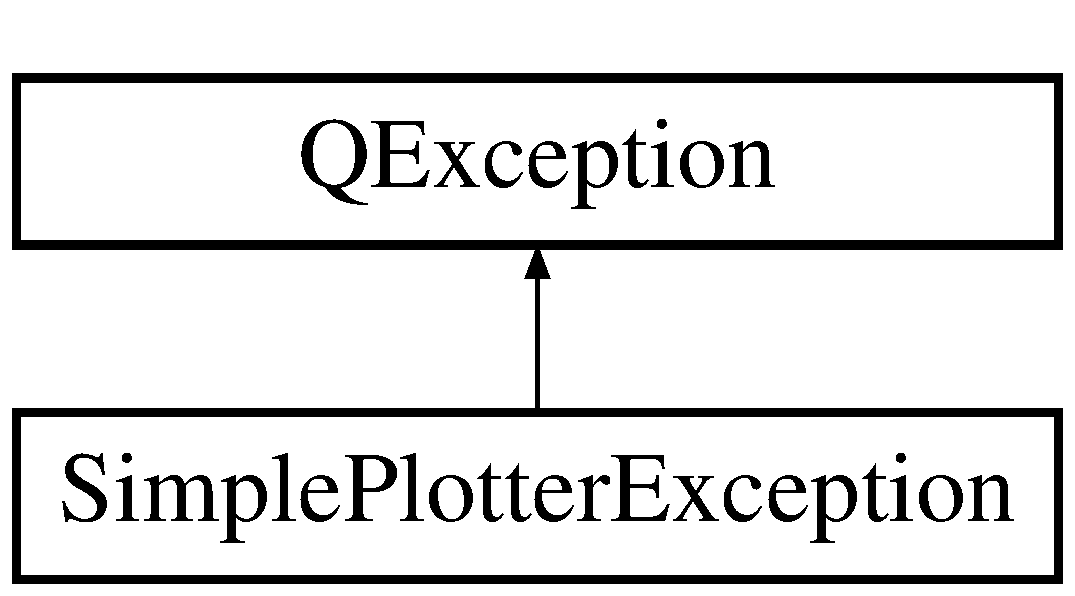
\includegraphics[height=2.000000cm]{class_simple_plotter_exception}
\end{center}
\end{figure}
\subsection*{Открытые члены}
\begin{DoxyCompactItemize}
\item 
\hyperlink{class_simple_plotter_exception_a6a0480aee21e9dfe7d06676ac01314ac}{Simple\+Plotter\+Exception} (Q\+String message)
\begin{DoxyCompactList}\small\item\em ����������� �� Q\+String. \end{DoxyCompactList}\item 
Q\+String \hyperlink{class_simple_plotter_exception_a234814fb4a3c88138929c7246d394418}{get\+Message} ()
\item 
\hyperlink{class_simple_plotter_exception_aa7c57585409e2480a9e152e2cdf289ca}{Simple\+Plotter\+Exception} (std\+::string message)
\begin{DoxyCompactList}\small\item\em ����������� �� std\+::string. \end{DoxyCompactList}\item 
\hyperlink{class_simple_plotter_exception_aa7d07eeb311c390164c2a35dbb804738}{Simple\+Plotter\+Exception} (char $\ast$message)
\begin{DoxyCompactList}\small\item\em ����������� �� char$\ast$. \end{DoxyCompactList}\end{DoxyCompactItemize}


\subsection{Подробное описание}
����� ���������� 

����������, ������������ ��� ��������� � ����������������� 

\subsection{Конструктор(ы)}
\index{Simple\+Plotter\+Exception@{Simple\+Plotter\+Exception}!Simple\+Plotter\+Exception@{Simple\+Plotter\+Exception}}
\index{Simple\+Plotter\+Exception@{Simple\+Plotter\+Exception}!Simple\+Plotter\+Exception@{Simple\+Plotter\+Exception}}
\subsubsection[{\texorpdfstring{Simple\+Plotter\+Exception(\+Q\+String message)}{SimplePlotterException(QString message)}}]{\setlength{\rightskip}{0pt plus 5cm}Simple\+Plotter\+Exception\+::\+Simple\+Plotter\+Exception (
\begin{DoxyParamCaption}
\item[{Q\+String}]{message}
\end{DoxyParamCaption}
)}\hypertarget{class_simple_plotter_exception_a6a0480aee21e9dfe7d06676ac01314ac}{}\label{class_simple_plotter_exception_a6a0480aee21e9dfe7d06676ac01314ac}


����������� �� Q\+String. 


\begin{DoxyParams}{Аргументы}
{\em message} & ����� ���������� \\
\hline
\end{DoxyParams}
\index{Simple\+Plotter\+Exception@{Simple\+Plotter\+Exception}!Simple\+Plotter\+Exception@{Simple\+Plotter\+Exception}}
\index{Simple\+Plotter\+Exception@{Simple\+Plotter\+Exception}!Simple\+Plotter\+Exception@{Simple\+Plotter\+Exception}}
\subsubsection[{\texorpdfstring{Simple\+Plotter\+Exception(std\+::string message)}{SimplePlotterException(std::string message)}}]{\setlength{\rightskip}{0pt plus 5cm}Simple\+Plotter\+Exception\+::\+Simple\+Plotter\+Exception (
\begin{DoxyParamCaption}
\item[{std\+::string}]{message}
\end{DoxyParamCaption}
)}\hypertarget{class_simple_plotter_exception_aa7c57585409e2480a9e152e2cdf289ca}{}\label{class_simple_plotter_exception_aa7c57585409e2480a9e152e2cdf289ca}


����������� �� std\+::string. 


\begin{DoxyParams}{Аргументы}
{\em message} & ����� ���������� \\
\hline
\end{DoxyParams}
\index{Simple\+Plotter\+Exception@{Simple\+Plotter\+Exception}!Simple\+Plotter\+Exception@{Simple\+Plotter\+Exception}}
\index{Simple\+Plotter\+Exception@{Simple\+Plotter\+Exception}!Simple\+Plotter\+Exception@{Simple\+Plotter\+Exception}}
\subsubsection[{\texorpdfstring{Simple\+Plotter\+Exception(char $\ast$message)}{SimplePlotterException(char *message)}}]{\setlength{\rightskip}{0pt plus 5cm}Simple\+Plotter\+Exception\+::\+Simple\+Plotter\+Exception (
\begin{DoxyParamCaption}
\item[{char $\ast$}]{message}
\end{DoxyParamCaption}
)}\hypertarget{class_simple_plotter_exception_aa7d07eeb311c390164c2a35dbb804738}{}\label{class_simple_plotter_exception_aa7d07eeb311c390164c2a35dbb804738}


����������� �� char$\ast$. 


\begin{DoxyParams}{Аргументы}
{\em message} & ����� ���������� \\
\hline
\end{DoxyParams}


\subsection{Методы}
\index{Simple\+Plotter\+Exception@{Simple\+Plotter\+Exception}!get\+Message@{get\+Message}}
\index{get\+Message@{get\+Message}!Simple\+Plotter\+Exception@{Simple\+Plotter\+Exception}}
\subsubsection[{\texorpdfstring{get\+Message()}{getMessage()}}]{\setlength{\rightskip}{0pt plus 5cm}Q\+String Simple\+Plotter\+Exception\+::get\+Message (
\begin{DoxyParamCaption}
{}
\end{DoxyParamCaption}
)}\hypertarget{class_simple_plotter_exception_a234814fb4a3c88138929c7246d394418}{}\label{class_simple_plotter_exception_a234814fb4a3c88138929c7246d394418}
\begin{DoxyReturn}{Возвращает}
����� ���������� 
\end{DoxyReturn}


Объявления и описания членов классов находятся в файлах\+:\begin{DoxyCompactItemize}
\item 
simpleplotterexception.\+h\item 
simpleplotterexception.\+cpp\end{DoxyCompactItemize}

\hypertarget{class_simple_plotter_scene}{}\section{Класс Simple\+Plotter\+Scene}
\label{class_simple_plotter_scene}\index{Simple\+Plotter\+Scene@{Simple\+Plotter\+Scene}}
Граф наследования\+:Simple\+Plotter\+Scene\+:\begin{figure}[H]
\begin{center}
\leavevmode
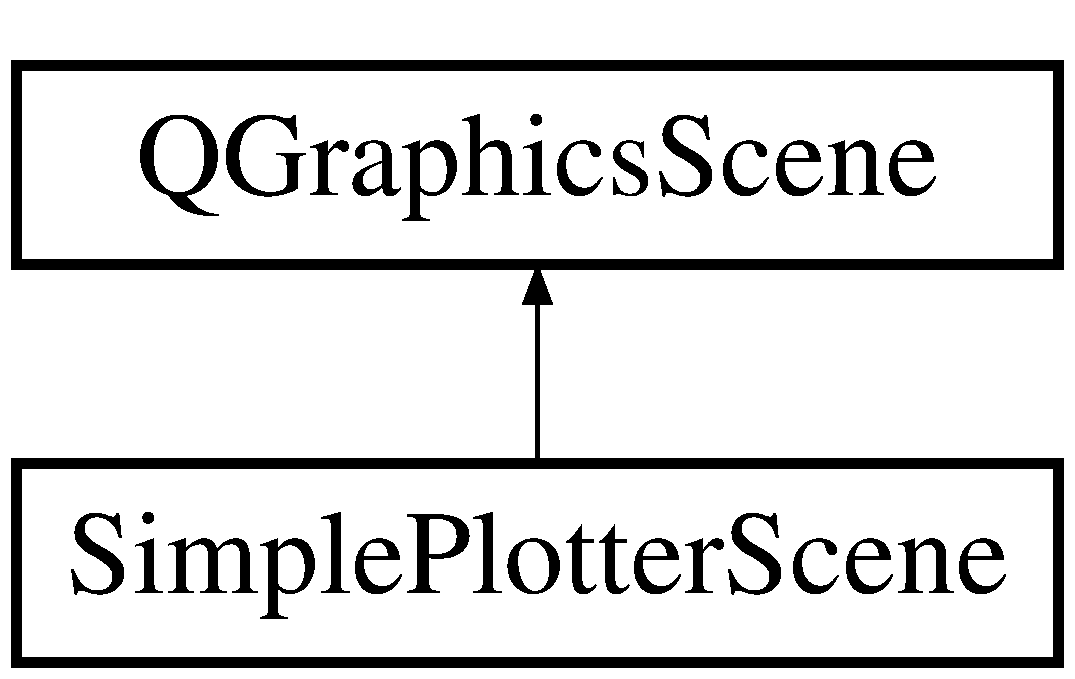
\includegraphics[height=2.000000cm]{class_simple_plotter_scene}
\end{center}
\end{figure}


Объявления и описания членов классов находятся в файлах\+:\begin{DoxyCompactItemize}
\item 
simpleplotterscene.\+h\item 
simpleplotterscene.\+cpp\end{DoxyCompactItemize}

\hypertarget{class_simple_plotter_view}{}\section{Класс Simple\+Plotter\+View}
\label{class_simple_plotter_view}\index{Simple\+Plotter\+View@{Simple\+Plotter\+View}}


�������� ����� �������  




{\ttfamily \#include $<$simpleplotterview.\+h$>$}

Граф наследования\+:Simple\+Plotter\+View\+:\begin{figure}[H]
\begin{center}
\leavevmode
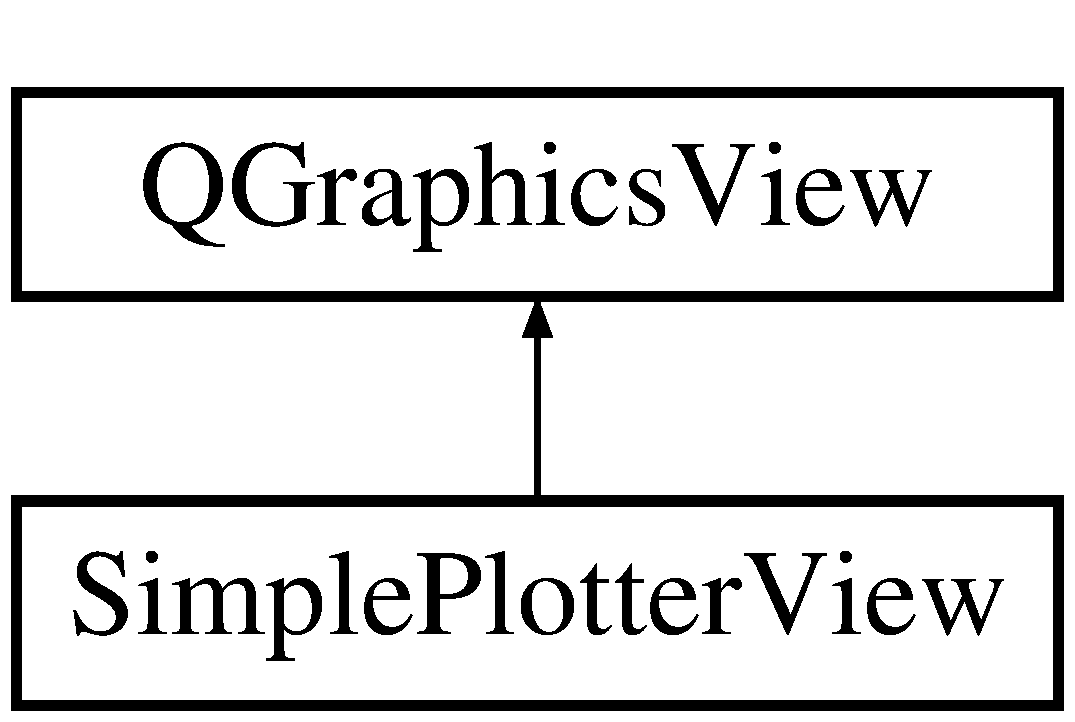
\includegraphics[height=2.000000cm]{class_simple_plotter_view}
\end{center}
\end{figure}
\subsection*{Открытые члены}
\begin{DoxyCompactItemize}
\item 
\hyperlink{class_simple_plotter_view_a4e9079ddecf20ade6a13c48f5c13a09e}{Simple\+Plotter\+View} (Q\+Widget $\ast$parent=0)
\begin{DoxyCompactList}\small\item\em ����������� \end{DoxyCompactList}\item 
\hyperlink{class_simple_plotter_view_ae04b23819fa8728ad605006c261cd102}{$\sim$\+Simple\+Plotter\+View} ()\hypertarget{class_simple_plotter_view_ae04b23819fa8728ad605006c261cd102}{}\label{class_simple_plotter_view_ae04b23819fa8728ad605006c261cd102}

\begin{DoxyCompactList}\small\item\em ���������� \end{DoxyCompactList}\item 
void \hyperlink{class_simple_plotter_view_a920ed0d07a22e2b537721b5acdd286e8}{append\+Plot} (\hyperlink{class_simple2_d_plot}{Simple2\+D\+Plot} a, Q\+Color color=Qt\+::red)
\begin{DoxyCompactList}\small\item\em �������� ����� ������ \end{DoxyCompactList}\item 
void \hyperlink{class_simple_plotter_view_a03a0c23480fdcb51b74832767aa2e822}{remove\+Plot} (std\+::string name)
\begin{DoxyCompactList}\small\item\em ������� ������ \end{DoxyCompactList}\end{DoxyCompactItemize}


\subsection{Подробное описание}
�������� ����� ������� 

�������� �����, ������� Q\+Graphics\+View 

\subsection{Конструктор(ы)}
\index{Simple\+Plotter\+View@{Simple\+Plotter\+View}!Simple\+Plotter\+View@{Simple\+Plotter\+View}}
\index{Simple\+Plotter\+View@{Simple\+Plotter\+View}!Simple\+Plotter\+View@{Simple\+Plotter\+View}}
\subsubsection[{\texorpdfstring{Simple\+Plotter\+View(\+Q\+Widget $\ast$parent=0)}{SimplePlotterView(QWidget *parent=0)}}]{\setlength{\rightskip}{0pt plus 5cm}Simple\+Plotter\+View\+::\+Simple\+Plotter\+View (
\begin{DoxyParamCaption}
\item[{Q\+Widget $\ast$}]{parent = {\ttfamily 0}}
\end{DoxyParamCaption}
)\hspace{0.3cm}{\ttfamily [explicit]}}\hypertarget{class_simple_plotter_view_a4e9079ddecf20ade6a13c48f5c13a09e}{}\label{class_simple_plotter_view_a4e9079ddecf20ade6a13c48f5c13a09e}


����������� 


\begin{DoxyParams}{Аргументы}
{\em parent} & ������������ ������ \\
\hline
\end{DoxyParams}


\subsection{Методы}
\index{Simple\+Plotter\+View@{Simple\+Plotter\+View}!append\+Plot@{append\+Plot}}
\index{append\+Plot@{append\+Plot}!Simple\+Plotter\+View@{Simple\+Plotter\+View}}
\subsubsection[{\texorpdfstring{append\+Plot(\+Simple2\+D\+Plot a, Q\+Color color=\+Qt\+::red)}{appendPlot(Simple2DPlot a, QColor color=Qt::red)}}]{\setlength{\rightskip}{0pt plus 5cm}void Simple\+Plotter\+View\+::append\+Plot (
\begin{DoxyParamCaption}
\item[{{\bf Simple2\+D\+Plot}}]{a, }
\item[{Q\+Color}]{color = {\ttfamily Qt\+:\+:red}}
\end{DoxyParamCaption}
)}\hypertarget{class_simple_plotter_view_a920ed0d07a22e2b537721b5acdd286e8}{}\label{class_simple_plotter_view_a920ed0d07a22e2b537721b5acdd286e8}


�������� ����� ������ 


\begin{DoxyParams}{Аргументы}
{\em a} & ������ ���� \hyperlink{class_simple2_d_plot}{Simple2\+D\+Plot}, �������� ���������� � ������� \\
\hline
{\em color} & ���� \\
\hline
\end{DoxyParams}
\index{Simple\+Plotter\+View@{Simple\+Plotter\+View}!remove\+Plot@{remove\+Plot}}
\index{remove\+Plot@{remove\+Plot}!Simple\+Plotter\+View@{Simple\+Plotter\+View}}
\subsubsection[{\texorpdfstring{remove\+Plot(std\+::string name)}{removePlot(std::string name)}}]{\setlength{\rightskip}{0pt plus 5cm}Simple\+Plotter\+View\+::remove\+Plot (
\begin{DoxyParamCaption}
\item[{std\+::string}]{name}
\end{DoxyParamCaption}
)}\hypertarget{class_simple_plotter_view_a03a0c23480fdcb51b74832767aa2e822}{}\label{class_simple_plotter_view_a03a0c23480fdcb51b74832767aa2e822}


������� ������ 


\begin{DoxyParams}{Аргументы}
{\em name} & ��� ������� \\
\hline
\end{DoxyParams}


Объявления и описания членов классов находятся в файлах\+:\begin{DoxyCompactItemize}
\item 
simpleplotterview.\+h\item 
simpleplotterview.\+cpp\end{DoxyCompactItemize}

\hypertarget{class_simple_plotter_widget}{}\section{Класс Simple\+Plotter\+Widget}
\label{class_simple_plotter_widget}\index{Simple\+Plotter\+Widget@{Simple\+Plotter\+Widget}}
Граф наследования\+:Simple\+Plotter\+Widget\+:\begin{figure}[H]
\begin{center}
\leavevmode
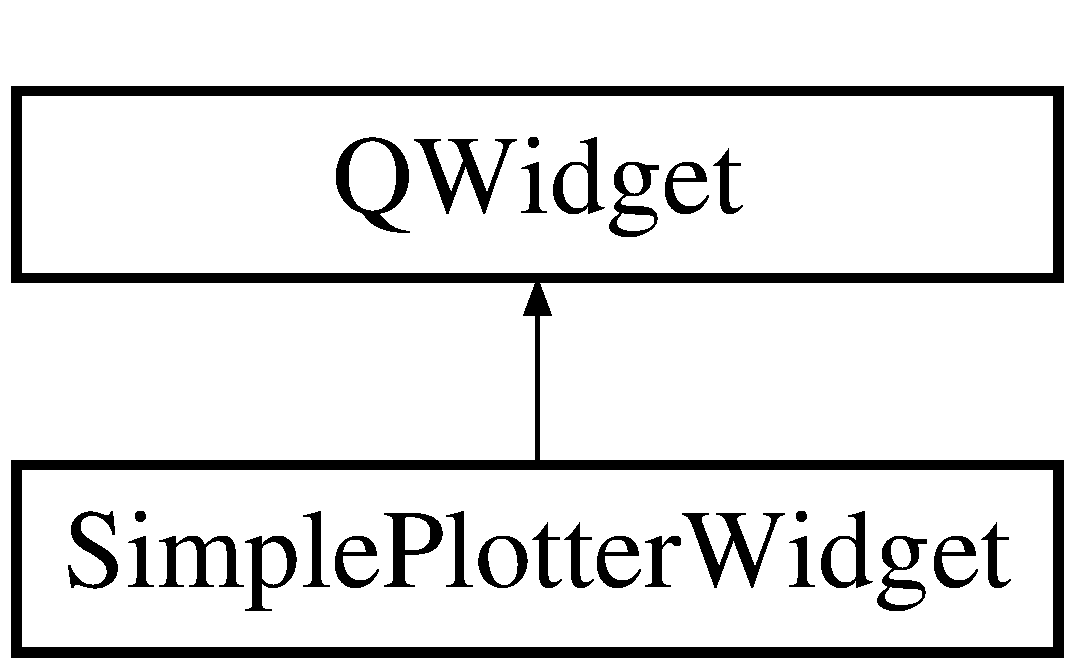
\includegraphics[height=2.000000cm]{class_simple_plotter_widget}
\end{center}
\end{figure}


Объявления и описания членов классов находятся в файлах\+:\begin{DoxyCompactItemize}
\item 
simpleplotterwidget.\+h\item 
simpleplotterwidget.\+cpp\end{DoxyCompactItemize}

%--- End generated contents ---

% Index
\backmatter
\newpage
\phantomsection
\clearemptydoublepage
\addcontentsline{toc}{chapter}{Алфавитный указатель}
\printindex

\end{document}
